\RequirePackage[l2tabu,orthodox]{nag}
\RequirePackage{fixltx2e}

\documentclass{beamer}

\usepackage{mflogo}
\usepackage{manfnt}
\usepackage{hieroglf}
\usepackage{marvosym}
\usepackage{wasysym}
\usepackage{url}

\title{A Brief Intro to \LaTeX{} and Friends}
\author{Peter H.\ Fr{\"o}hlich\\
\texttt{phf@cs.jhu.edu}}
\date{February 12, 2015}

\begin{document}

\frame{
\titlepage
}

\frame{
\frametitle{Outline}
\tableofcontents
}

\section{Motivation}

\frame{
\begin{center}
\Huge\smiley\\\textbf{Motivation}
\end{center}
}

\frame{
  \frametitle{Cute Mascot!}
  \begin{center}
    
\includegraphics[height=0.8\textheight]{lion}\\
    {\tiny\url{http://www.ctan.org/lion/}}
  \end{center}
}

\section{History}

\frame{
\begin{center}
\Huge\textpmhg{\Ha\Hv\Hman}\\\textbf{History}
\end{center}
}

\frame{
  \frametitle{Donald Knuth}
  \begin{center}
    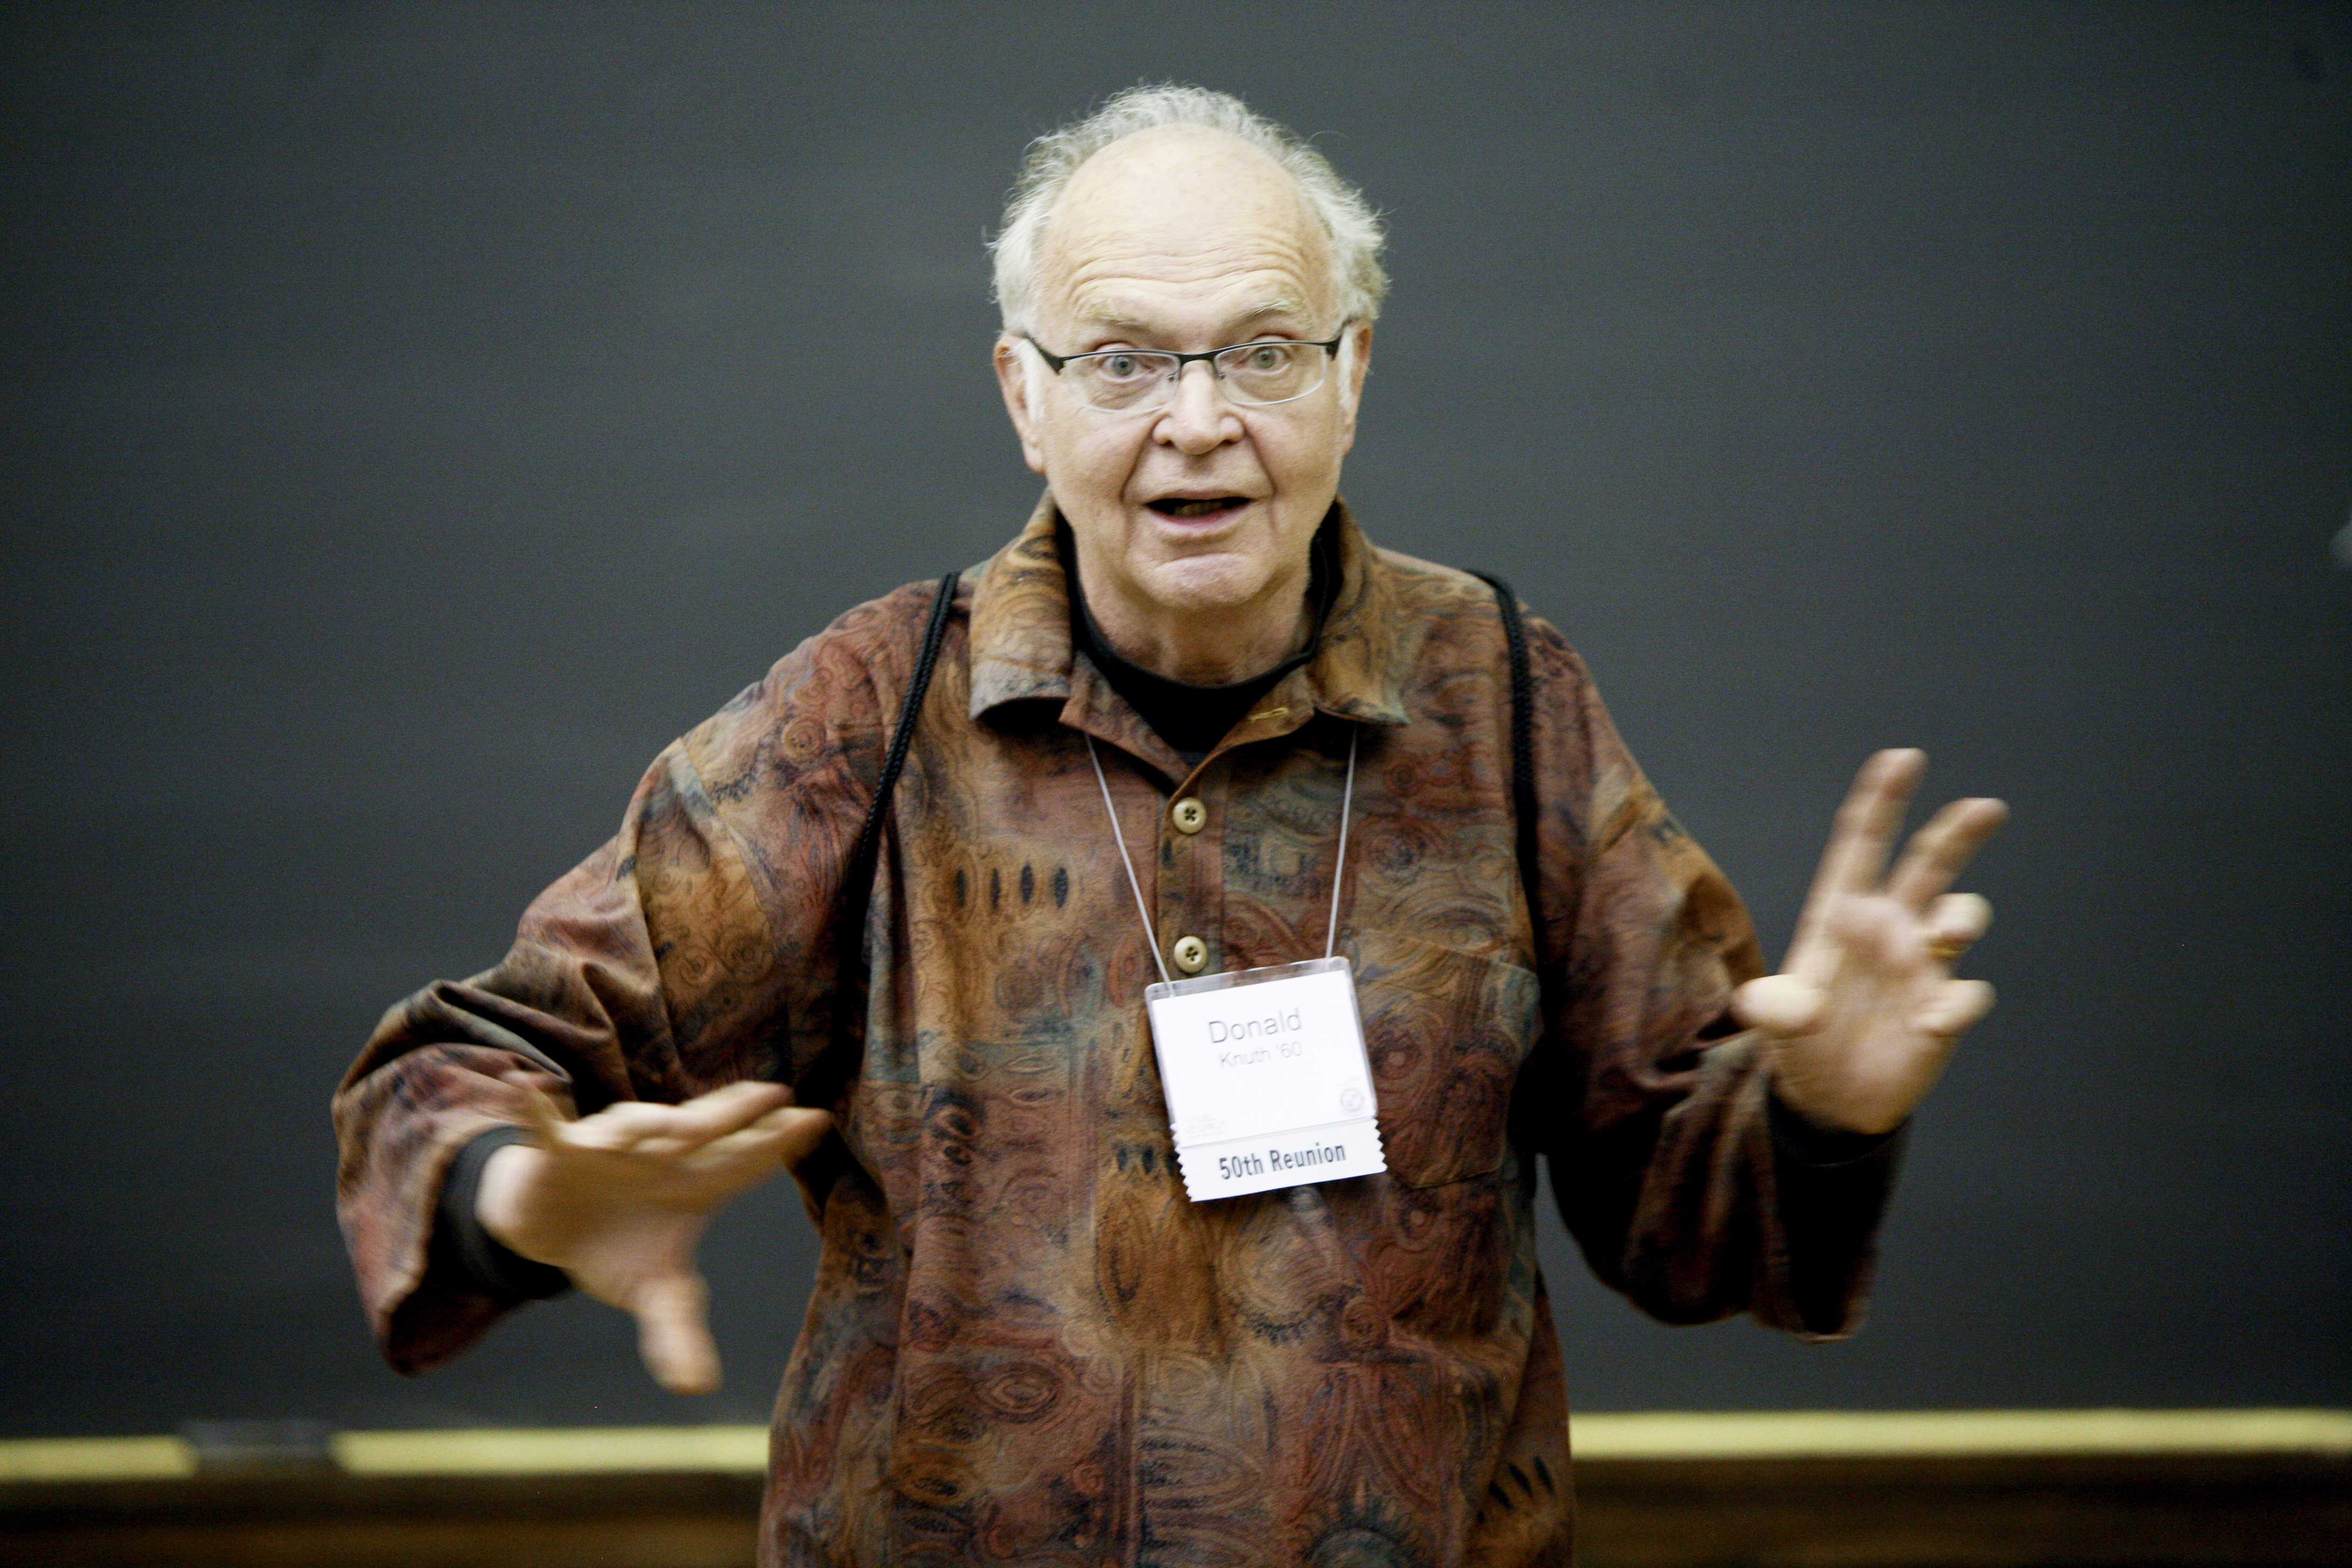
\includegraphics[width=\textwidth]{knuth}\\
    {\tiny\url{http://www-cs-faculty.stanford.edu/~uno/graphics.html}}
  \end{center}
}

\frame{
  \frametitle{Donald Knuth}
  \begin{itemize}
    \item ACM Turing Award (1974)
    \begin{itemize}
      \item \emph{For his major contributions to the
        analysis of algorithms and the design of
        programming languages\dots}
    \end{itemize}
    \item Wanted to produce more beautiful books, himself.
    \begin{itemize}
      \item Studied typography and font design, in depth.
      \item Lots of interesting algorithms, for example hyphenation.
      \item Developed \TeX{} and \MF{} languages and tools.
      \item Documented (with complete source) in five books.
    \end{itemize}
    \item Version numbers converge to \(\pi\) and \(e\) on Knuth's death.
    \begin{itemize}
      \item Designed for ``eternity,'' not necessarily ``modernity.''
    \end{itemize}
  \end{itemize}
}

\frame{
  \frametitle{Leslie Lamport}
  \begin{center}
    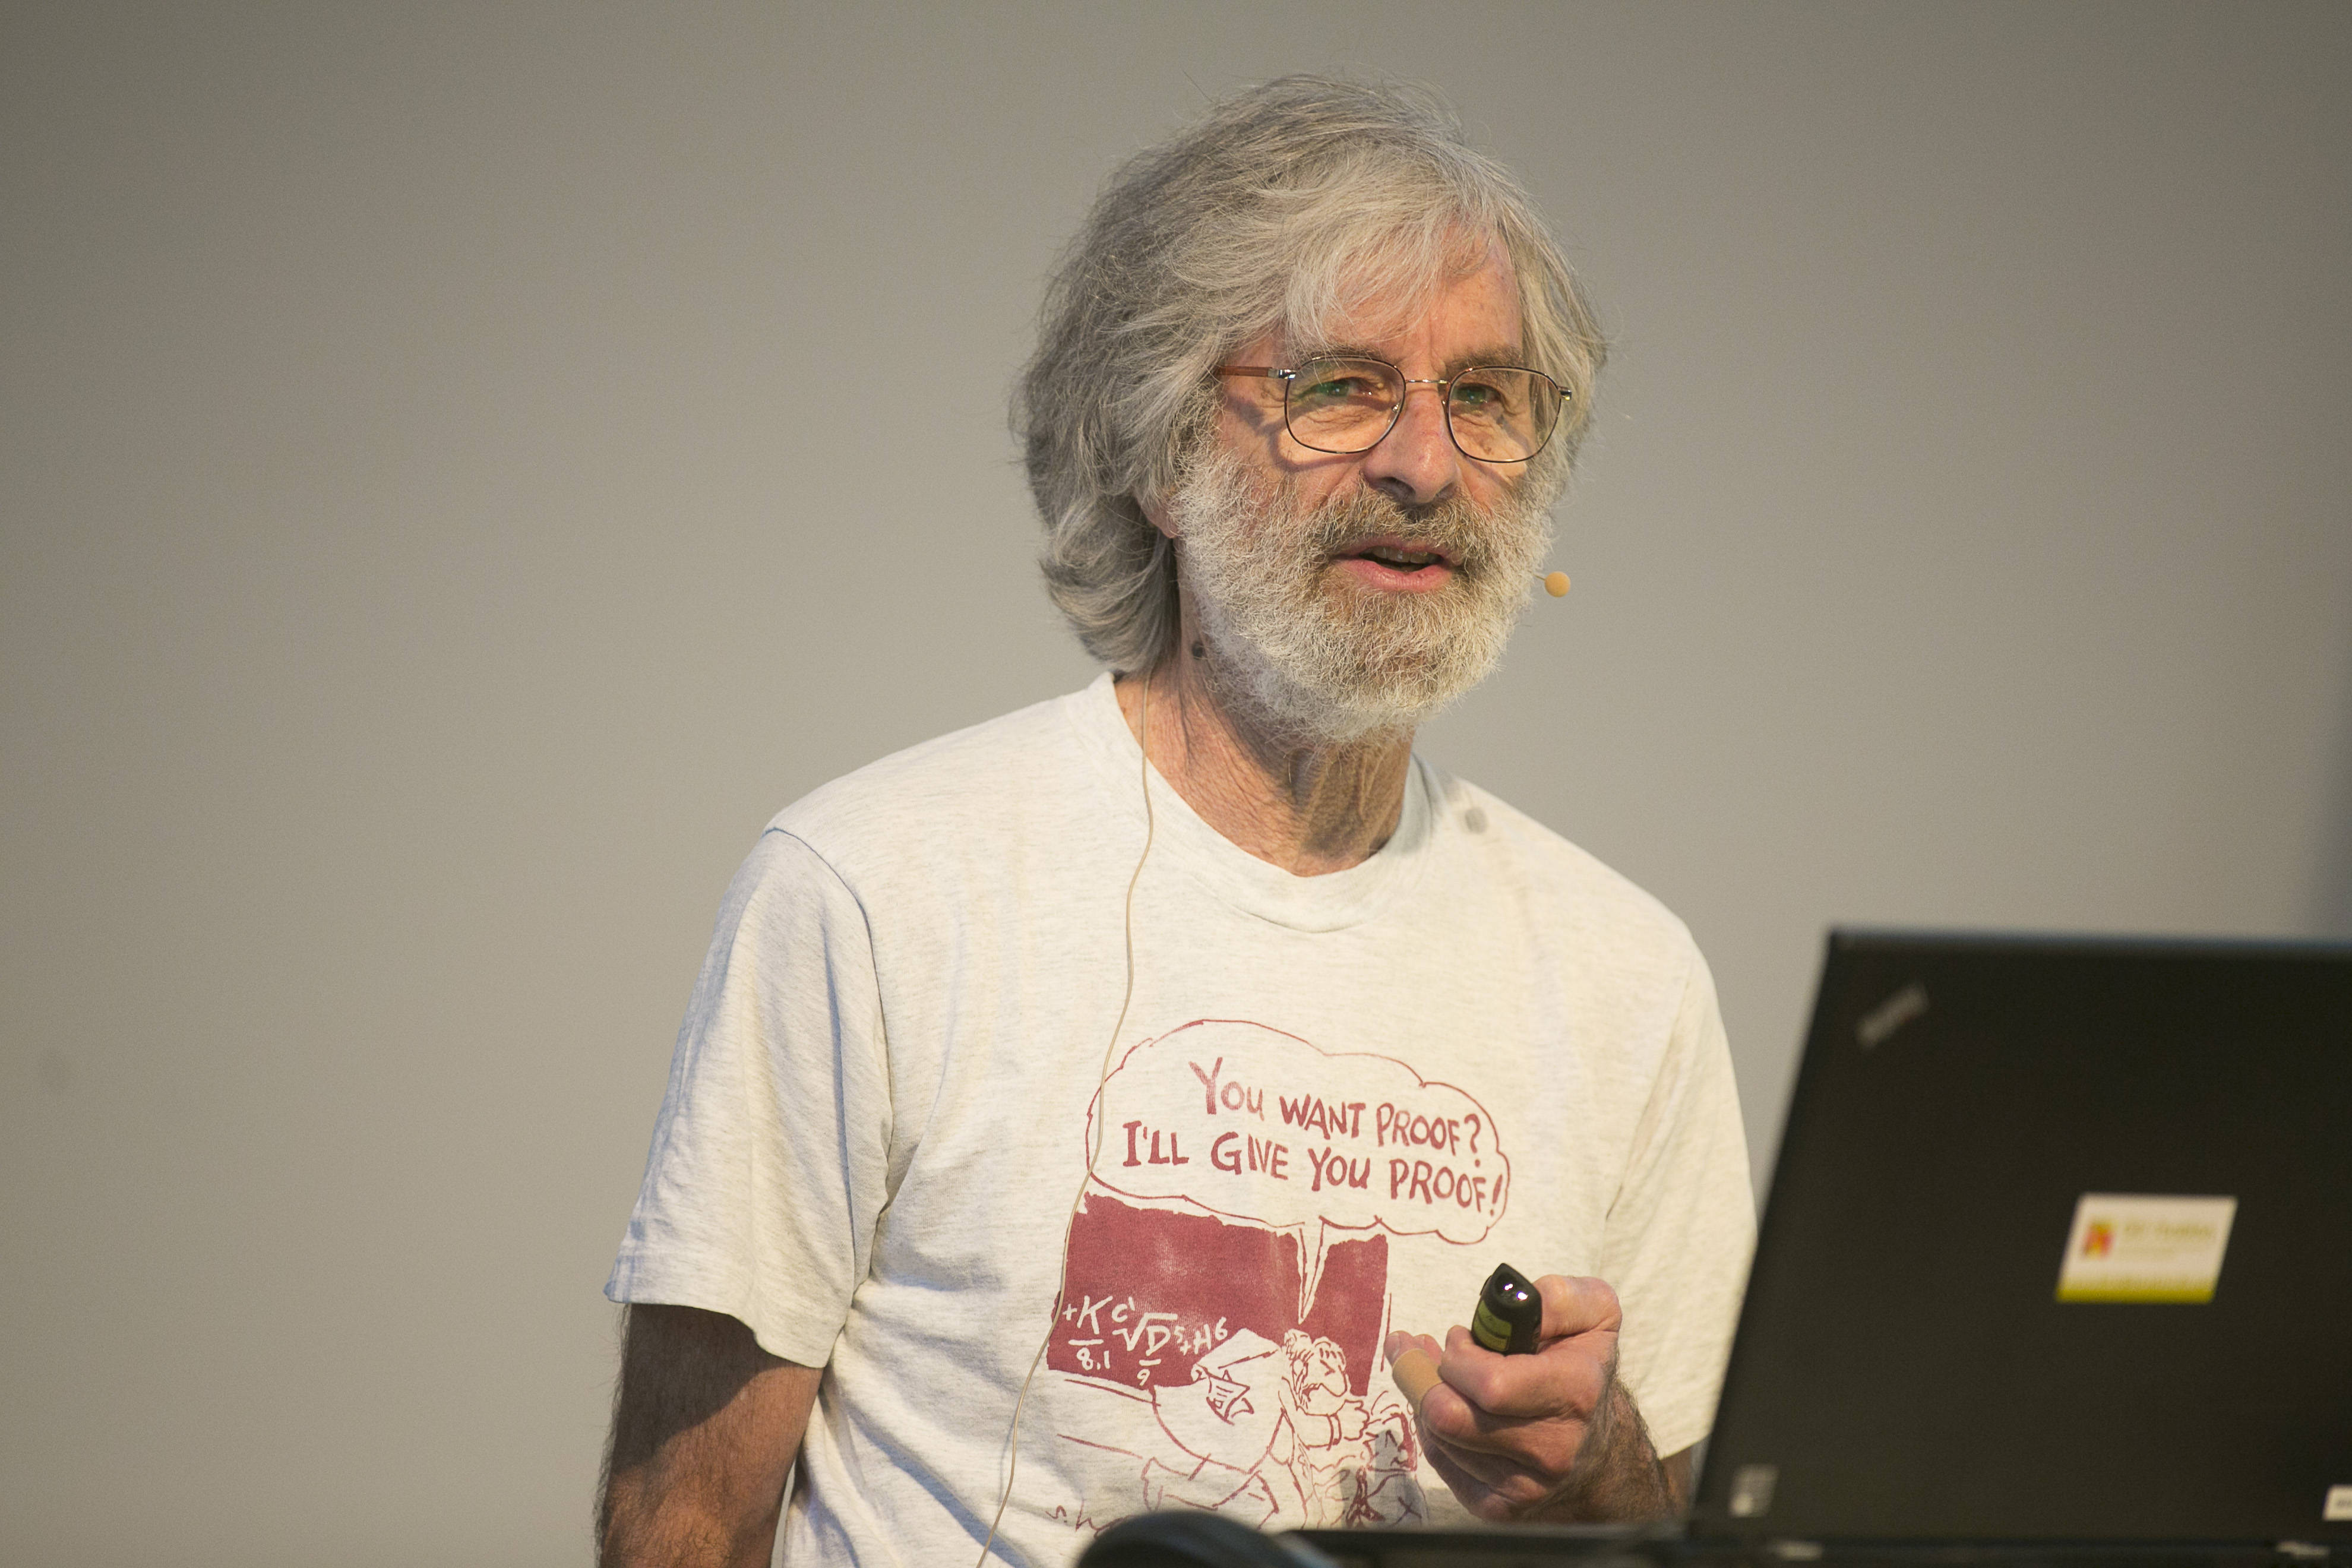
\includegraphics[width=\textwidth]{lamport}\\
    {\tiny\url{http://www.scilogs.com/hlf/writing-for-mathematical-clarity/}}
  \end{center}
}

\frame{
  \frametitle{Leslie Lamport}
  \begin{itemize}
    \item ACM Turing Award (2013)
    \begin{itemize}
      \item \emph{For fundamental contributions to the
        theory and practice of distributed and
        concurrent systems\dots}
    \end{itemize}
    \item Wanted to use \TeX{} to write a book on concurrency.
    \begin{itemize}
      \item Found \TeX{} too low-level, wanted more structure.
      \item Developed \LaTeX{} macro package to that end.
      \item Never wrote that concurrency book\dots{}
      \begin{itemize}
        \item Did write a \LaTeX{} book! :-)
      \end{itemize}
    \end{itemize}
    \item Since taken over by a ``cast of thousands'' in \LaTeXe{}.
    \begin{itemize}
      \item Quite different from Lamport's original if you look closely.
      \item Also emphasizes stability and backwards-compatibility.
    \end{itemize}
  \end{itemize}
}

\section{Warnings}

\frame{
\begin{center}
\Huge\textdbend{}\\\textbf{Warnings}
\end{center}
}

\frame{
  \frametitle{Warnings}
  \begin{itemize}
    \item \LaTeX{} can be a bit frustrating when you start out.
    \begin{itemize}
      \item Just trust that once you get it, you won't go back.
      \item Keep it simple, focus on content not presentation.
    \end{itemize}
    \item There's a huge ecosystem out there!
    \begin{itemize}
      \item Almost everything exists (but it might be 20 years old).
      \item Can be difficult to find exactly what you're looking for.
      \item But it's generally a pretty friendly community.
    \end{itemize}
    \item Packages may seem like modules, but they are really not.
    \begin{itemize}
      \item Subtle interactions between different packages.
      \item Order of ``import'' can matter even though it shouldn't.
      \item It's almost all text-macros in the end, act accordingly!
    \end{itemize}
    \item Use \texttt{fixltx2e} and \texttt{nag} as I'll show you!
    \begin{itemize}
      \item And watch for \texttt{nag} warnings, otherwise it won't help you.
    \end{itemize}
  \end{itemize}
}

\section{Demos}

\frame{
\begin{center}
\Huge\Keyboard{} \ComputerMouse\\\textbf{Demos}
\end{center}
}

\section{Questions?}

\frame{
\begin{center}
\Huge\frownie{}\\\textbf{Questions?}
\end{center}
}

\end{document}
